%-----------------------------------------------------------
% LaTeX template for University of Warwick exams
%-----------------------------------------------------------

\usepackage{fancyeq}
\usepackage{tikz}
\usetikzlibrary{automata, positioning, arrows}
\makeatletter
\expandafter\providecommand\expandafter*\csname ver@framed.sty\endcsname
{2003/07/21 v0.8a Simulated by exam}
\makeatother
\usepackage{framed}
\usepackage{xcolor}
\usepackage{minted}
\usepackage[
backgroundcolor = white
, hidealllines=true
]{mdframed}

\surroundwithmdframed{minted}
\usemintedstyle{bw}

\setminted[text]{fontsize=\small}
\setminted[haskell]{fontsize=\small}
\setminted[bash]{fontsize=\small}
\newcommand{\haskellIn}[1]{\mintinline[fontsize=\small]{text}{#1}}
\newcommand{\bashIn}[1]{\mintinline[fontsize=\small]{bash}{#1}}

\usepackage[]{FiraSans}

\usepackage{mathpazo}
\linespread{1.05}         % Palatino needs more leading (space between lines)
\usepackage[T1]{fontenc}

\usepackage{multicol}

%\usepackage[nomap]{FiraMono}

% configure the heading 
\ModuleName{Functional Programming}
\ExamPeriod{Summer 2019}
\TimeAllowed{2 hours}
\QuestionInstructions{Answer \textbf{FOUR} questions.}
\OtherInstructions{Read carefully the instructions on the answer book and make sure that the particulars required are entered on \textbf{each} answer book. \\

No calculators are allowed. A copy of the Haskell Prelude is given in the Appendix.}

\usepackage[nomap]{FiraMono}

\usepackage{microtype}
\DisableLigatures[f]{encoding = *, family = tt* }

\begin{document}
	\MakeHeading
	
	\begin{questions}
		%%% Question 1 - - - - - - - - - - - - - - - - - - - - - - - - - - - - - -
\question This question is about functional programming as a programming paradigm.
\begin{parts}
	
	\part For each of the following Haskell expressions, reduce it to its normal form.
	
	\begin{subparts}
		
		\subpart[1] \haskellIn{head "Witter" : tail "Virus"} \droppoints 
		
		\begin{solution}
		\emph{Comprehension.} \haskellIn{"Wirus"} 
		\end{solution}
	
		\subpart[1] \haskellIn{take (fst (3,9002)) (repeat "Blue")}  \droppoints
		
		\begin{solution}
		\emph{Comprehension.} \haskellIn{["Blue", "Blue", "Blue"]}
		\end{solution}
	
		\subpart[1] \haskellIn{foldr (:) [] (Just 108)}  \droppoints
		
		\begin{solution}
		\emph{Comprehension.} \haskellIn{[108]}
		\end{solution}
	
		\subpart[1] \haskellIn{fmap (+2) (\x -> x*5) 4} \droppoints
		
		\begin{solution}
		\emph{Comprehension.} \haskellIn{22}
		\end{solution}
	
		\subpart[1] \haskellIn{foldl (\r x -> fmap (x:) r ++ r) [[]] "abc"} \droppoints
		
		\begin{solution}
		\emph{Comprehension.}\\ \haskellIn{["cba","cb","ca","c","ba","b","a",""]}
		\end{solution}
	\end{subparts}
	
	\part For each of the following expressions, choose \emph{all} permissible types from the options that are listed. There is \emph{at least} one correct option for each expression.
	
	\begin{subparts}
		
    	\subpart[1] \haskellIn{show 24} \droppoints
    	
	    \begin{enumerate}
	    	\item \haskellIn{[Char]}
	    	\item \haskellIn{Show a => a -> String}
	    	\item \haskellIn{(Show a, Num a) => a -> String}
	    	\item \haskellIn{(Show a, Num a) => a -> [Char]}
	    	\item \haskellIn{String}
	    \end{enumerate}
    
		\begin{solution}
			\emph{Comprehension.} 1,5
		\end{solution}
	
    	\subpart[1] \haskellIn{[(1, "Angel Attack"), (2, "The Beast")]} \droppoints
    	
	    \begin{enumerate}
	    	\item \haskellIn{Num a => [(a, String), (a, String)]}
	    	\item \haskellIn{Num a => [(a, String)]}
	    	\item \haskellIn{[(Int, String)]}
	    	\item \haskellIn{[(Integer, String)]}
	    	\item \haskellIn{Num a => [(a, [Char])]}
	    \end{enumerate}
    
	    \begin{solution}
	   		\emph{Comprehension.} 2,3,4,5
	    \end{solution}
    
    	\ifprintanswers \pagebreak \else \fi
    
    	%\ifprintanswers \else \pagebreak \fi
    	
    	\subpart[1] \haskellIn{\a b c d -> a (b d) c} \droppoints
    	
	    \begin{enumerate}
	    	\item \haskellIn{(a -> a -> a) -> (a -> a) -> a -> a -> a}
	    	\item \haskellIn{(a -> b -> a) -> (d -> a) -> b -> d -> a}
	    	\item \haskellIn{(d -> b -> c) -> (a -> d) -> b -> a -> c}
	    	\item \haskellIn{(a -> a -> c) -> (d -> a) -> a -> d -> c}
	    	\item \haskellIn{(a -> b -> c) -> (d -> a) -> b -> d -> c}
	    \end{enumerate}
    
	    \begin{solution}
	    	\emph{Comprehension.} 1,2,3,4,5
	    \end{solution}
    
		\subpart[1] \haskellIn{\f -> fmap (f (fmap id)) []} \droppoints
		
		\begin{enumerate}
			\item \haskellIn{Functor f => ((f b -> f c) -> a -> c) -> [c]}
			\item \haskellIn{Functor f => ([b] -> [b] -> a -> c) -> f c}
			\item \haskellIn{Functor f => (([b] -> [b]) -> a -> c) -> f c}
			\item \haskellIn{Functor f => ((f b -> f b) -> a -> c) -> [c]}
			\item \haskellIn{Functor f => ((f b -> f b) -> a -> c) -> f c}
		\end{enumerate}
	
		\begin{solution}
			\emph{Comprehension.} 4
		\end{solution}
	
		%\ifprintanswers \pagebreak \else \fi
		
    	\subpart[1] \haskellIn{\f z xs -> foldr (\b g x -> g (f x b)) id xs z} \droppoints 
    	
	    \begin{enumerate}
	    	\item \haskellIn{(a -> b -> a) -> a -> [b] -> a}
	    	\item \haskellIn{(a -> b -> b) -> b -> [a] -> b}
	    	\item \haskellIn{Foldable t => (a -> b -> b) -> b -> t a -> b}
	    	\item \haskellIn{Foldable t => (b -> a -> b) -> b -> t a -> b}
	    	\item \haskellIn{Foldable t => (b -> a -> c) -> b -> t a -> c}
	    \end{enumerate}
    
	    \begin{solution}
	    	\emph{Comprehension.} 1,4
	    \end{solution}
	\end{subparts}

	\ifprintanswers \else \pagebreak \fi

	\part[3] Consider the following definition of the list difference operator \haskellIn{(\\)}:
	\begin{small}
	\begin{verbatim}
	(\\) :: Eq a => [a] -> [a] -> [a]
	xs \\ []     = xs 
	xs \\ (y:ys) = delete y (xs \\ ys)
	\end{verbatim}
	\end{small}
	
	Define a function \haskellIn{diff} which is equivalent to \haskellIn{(\\)}, but is defined using \haskellIn{foldl} instead of explicit recursion. \droppoints 
	
	\begin{solution}
	\emph{Application.} One possible answer is:
	\begin{verbatim}
	diff = foldl (flip delete)
	\end{verbatim}
	\end{solution}
\part  \label{part:sum}
\begin{subparts}
\subpart[3] \label{part:strict} Trace how \haskellIn{diff "abbc" "bd"} would be evaluated in a language with \emph{call-by-value} semantics. \droppoints
\begin{solution}
\emph{Comprehension.}
\begin{small}
\begin{verbatim}
   diff "abbc" "bd"
=> foldl (flip delete) "abbc" "bd"
=> foldl (flip delete) (flip delete "abbc" 'b') "d"
=> foldl (flip delete) "ac" "d"
=> foldl (flip delete) (flip delete "ac" 'd') ""
=> foldl (flip delete) "ac" ""
=> "ac"
\end{verbatim}
\end{small}
\end{solution}
\subpart[3] \label{part:lazy} Trace how \haskellIn{diff "abbc" "bd"} would be evaluated in a language with \emph{call-by-name} semantics. You should assume that the value of this expression is required by some other part of the program. \droppoints
\begin{solution} \emph{Comprehension.}
\begin{small}
\begin{verbatim}
diff "abbc" "bd"
=> foldl (flip delete) "abbc" "bd"
=> foldl (flip delete) (flip delete "abbc" 'b') "d"
=> foldl (flip delete) (flip delete 
     (flip delete "abbc" 'b') 'd') ""
=> flip delete (flip delete "abbc" 'b') 'd'
=> flip delete "ac" 'd'
=> "ac"
\end{verbatim}
\end{small}
\end{solution}
\subpart[6] Consider the following, well known definition which represents the infinite list of fibonacci numbers:
\begin{small}
	\begin{verbatim}
	fibs :: [Integer]
	fibs = 1 : 1 : zipWith (+) fibs (tail fibs)
	\end{verbatim}
\end{small}
Using relevant terminology and with reference to \emph{sharing}, explain why $n$-many elements of this list can be computed in linear time with respect to $n$. \droppoints
\begin{solution} \emph{Comprehension.}
Definitions are represented by \emph{closures} (stored on the heap) and pointers to them are then passed to functions as arguments. Sharing is an optimisation which allows closures to be \emph{updated} with their result once they have been evaluated provided that the closure (definition) has no parameters, meaning they only have to be evaluated once. The Haskell compiler rewrites the above definition to something like:
\begin{verbatim}
fibs :: [Integer]
fibs = let xs = 1 : ys 
           ys = zipWith (+) fibs zs
           zs = tail fibs
       in 1 : xs
\end{verbatim} 
Each definition corresponds to a closure and none of them have any parameters. In particular, \haskellIn{ys} and \haskellIn{zs} can be updated with the results of evaluating their respective operations. Since variables are pointers to those closures, they will see the results once they have been evaluated once and do not need to perform the same work again.
\end{solution}
\end{subparts}
\end{parts}

		%%% Question 2 - - - - - - - - - - - - - - - - - - - - - - - - - - - - - -
\question This question is about recursive and higher-order functions.
\begin{parts}
	\part[4] Define a function 
	
	\begin{center}
		\haskellIn{isPrime :: Integer -> Bool}
	\end{center} 

	which given an integer value, determines whether it is a prime number. For example, \haskellIn{isPrime 3} should evaluate to \haskellIn{True}. \droppoints
	
	\begin{solution}
	\emph{Application.} A simple solution using a list comprehension is:
	\begin{verbatim}
	isPrime :: Integer -> Bool 
	isPrime n = null [x | x <- [2..n-1], n `mod` x == 0]
	\end{verbatim}
	\end{solution}

	\part[2] With the help of \haskellIn{isPrime}, write a definition 
	
	\begin{center}
		\haskellIn{primes :: [Integer]} 
	\end{center}

	which represents the \emph{infinite} list of prime numbers. For example, the expression \haskellIn{take 4 primes} should evaluate to \haskellIn{[2,3,5,7]}. \droppoints
	
	\begin{solution} \emph{Application.}
	\begin{verbatim}
	primes :: [Integer]
	primes = [n | n <- [2..], isPrime n]
	\end{verbatim}
	\end{solution}

	\part Two words are anagrams of each other if they are made up of the same characters. For example, \haskellIn{"team"} and \haskellIn{"meta"} are anagrams of each other. One method for determining whether two words are anagrams of each other is to assign a unique prime number to each character in the alphabet, map each character in a given word to its corresponding prime number, and then calculate the product of all those numbers. The product of two or more prime numbers is guaranteed to be unique for those prime factors so if two words result in the same product, they must be anagrams of each other. 

	\begin{subparts}
		\subpart[4] Write a function 
		
		\begin{center}
			\haskellIn{toPrime :: Char -> Integer}
		\end{center}
	
		which maps each character in the alphabet to a unique prime number. For example, \haskellIn{toPrime 'A'} and \haskellIn{toPrime 'a'} could evaluate to \haskellIn{2} while \haskellIn{toPrime 'C'} could evaluate to \haskellIn{5}. \emph{Hint}: the \haskellIn{ord :: Char -> Int} function maps characters to their corresponding integer value in the ASCII encoding.  \droppoints 
		
		\begin{solution}
			\emph{Application.} 
			\begin{verbatim}
			toPrime :: Char -> Integer
			toPrime c = primes !! (ord (toUpper c) - ord 'A')
			\end{verbatim}
		\end{solution}
		
		\subpart[3] With the help of \haskellIn{toPrime}, define a function
		
		\begin{center}
			\haskellIn{score :: String -> Integer}
		\end{center}
	
		which calculates the product of all the prime numbers for all the characters in the input string. For example, assuming that \haskellIn{toPrime} maps \haskellIn{'a'} to \haskellIn{2}, \haskellIn{'b'} to \haskellIn{3}, \haskellIn{'c'} to \haskellIn{5} and so on, \haskellIn{score "team"} should evaluate to \haskellIn{64042}. \droppoints 
		
		\begin{solution}
			\emph{Application.} 
			\begin{verbatim}
			score :: String -> Integer
			score = product . map toPrime
			\end{verbatim}
		\end{solution}
	
		\subpart[2] With the help of \haskellIn{score}, define a function 
		
		\begin{center}
			\haskellIn{isAnagram :: String -> String -> Bool}
		\end{center}
	
		which determines whether two \haskellIn{String} values are anagrams of each other. For example, \haskellIn{isAnagram "team" "meta"} should evaluate to \haskellIn{True}. \droppoints 
	
		\begin{solution}
			\emph{Application.} 
			\begin{verbatim}
			isAnagram :: String -> String -> Bool
			isAnagram xs ys = score xs == score ys
			\end{verbatim}
		\end{solution}
	
		\subpart[5] With the help of the previous definitions, define a function
		
		\begin{center}
			\haskellIn{anagrams :: [String] -> [(String, [String])]}
		\end{center}
	
		which, given a list of \haskellIn{String} values representing a list of words, returns a list of the same size in which every input word is mapped to a list of its anagrams. For example: \\[1mm]
		\haskellIn{anagrams ["team", "meta", "meat", "late"]} \\
		\haskellIn{=> [("team",["meta","meat"]),("meta",["team","meat"]),} \\
		\haskellIn{    ("meat",["team","meta"]),("late",[])]} \droppoints 
	
		\begin{solution}
			\emph{Application.} 
			\begin{verbatim}
			anagrams :: [String] -> [(String, [String])]
			anagrams xs = map (go xs) xs 
			  where go ys x = (x, [y | y <- ys, 
			                           isAnagram x y, x /= y])
			\end{verbatim}
		\end{solution}
	
		\ifprintanswers \else \pagebreak \fi
	
		\subpart[5] With the help of the previous definitions, define a function
		
		\begin{center}
			\haskellIn{subgrams :: [String] -> [(String, [String])]}
		\end{center}
	
		which behaves like \haskellIn{anagrams}, except it also considers words which do not use every character from the original word. For example:\\[1mm]
		\haskellIn{subgrams ["team", "meta", "eat", "tea"]} \\
		\haskellIn{=> [("team",["meta","eat","tea"]),} \\
		\haskellIn{ ("meta",["team","eat","tea"]),}\\
		\haskellIn{    ("eat",["tea"]),("tea",["eat"])]} \droppoints 
		
		\begin{solution}
			\emph{Application.}
			\begin{verbatim}
			subgrams :: [String] -> [(String, [String])]
			subgrams xs = map (go xs) xs 
			  where go ys x = (x, nub [y | y <- ys, 
			                               w <- subsequences x, 
			                               w /= [], 
			                               isAnagram y w, 
			                               x /= y])
			
			\end{verbatim}
		\end{solution}
		
	\end{subparts}

\end{parts}
 
		
%%% Question 3 - - - - - - - - - - - - - - - - - - - - - - - - - - - - - -
\question This question is about user-defined types and type classes.
\begin{parts}
	
	\part Consider a variant of rose trees where elements are stored in nodes rather than leaves such that, for example, the following is a valid definition:
	\begin{small}
		\begin{verbatim}
		tree :: Tree String 
		tree = Node "Sakura" [Node "Rubber" []]
		\end{verbatim}
	\end{small}
	
	\begin{subparts}
		
		\subpart[3] Give a suitable definition for the \haskellIn{Tree} type. \droppoints 
		
		\begin{solution}
			\emph{Application.}
			\begin{small}
				\begin{verbatim}
				data Tree a = Node a [Tree a]
				\end{verbatim}
			\end{small}
		\end{solution}
	
		\subpart[1] A collection of trees is referred to as a \emph{forest}. Define a suitable \emph{type alias} for \haskellIn{Forest a} which represents zero or more trees of  elements of type \haskellIn{a}. \droppoints 
		
		\begin{solution}
			\emph{Application.}
			\begin{small}
				\begin{verbatim}
				type Forest a = [Tree a]
				\end{verbatim}
			\end{small}
		\end{solution}
	
		\subpart[4] The \haskellIn{Tree} type is a functor. Define a suitable instance of Haskell's \haskellIn{Functor} type class for it. Your solution should obey the functor laws, although you do not need to prove this. \droppoints 
		
		\begin{solution}
			\emph{Application.} 
			\begin{small}
				\begin{verbatim}
				instance Functor Tree where 
				     fmap f (Node x ts) = Node (f x) (fmap (fmap f) ts)
				\end{verbatim}
			\end{small}
		\end{solution}
	
		\subpart[4] Define a suitable instance of Haskell's \haskellIn{Foldable} type class for the \haskellIn{Tree} type.  \droppoints 
		
		\begin{solution}
			\emph{Application.}
			\begin{small}
				\begin{verbatim}
				instance Foldable Tree where 
				  foldr f z (Node x ts) = 
				    f x (foldr (\t r -> foldr f r t) z ts)
				\end{verbatim}
			\end{small}
		\end{solution} 
		
	\end{subparts}

	\part A zipper is a purely functional data structure which can be used to efficiently traverse another data structure if the same element needs to be accessed repeatedly or element access is relative to the last-accessed element by allowing a particular element of the data structure to be ``focused''. Suppose that we have an implementation of binary trees as follows:
	\begin{small}
		\begin{verbatim}
		data BinTree a = BinLeaf a | BinNode (BinTree a) (BinTree a)
		\end{verbatim}
	\end{small}
	
	\begin{subparts}
		
		\subpart[2] Define an algebraic data type named \haskellIn{Direction} so that it has two constructors with the following types:\\
		\haskellIn{L :: BinTree a -> Direction a} \\
		\haskellIn{R :: BinTree a -> Direction a} \droppoints 
		
		\begin{solution}
			\emph{Application.}
			\begin{small}
				\begin{verbatim}
				data Direction a = L (BinTree a) | R (BinTree a)
				\end{verbatim}
			\end{small}
		\end{solution}
	
		\subpart[1] A zipper data structure for \haskellIn{BinTree} values can then be defined as:
		 
		\begin{small}
			\begin{verbatim}
			data BinZipper a = Pos [Direction a] (BinTree a)
			\end{verbatim}
		\end{small}
	
		What is the type of \haskellIn{Pos}? \droppoints
		
		\begin{solution}
			\emph{Comprehension.}\\
			\haskellIn{Pos :: [Direction a] -> BinTree a -> BinZipper a}
		\end{solution}
	
		\subpart[1] The definition of the \haskellIn{BinZipper} type above can be used to represent a position within a binary tree, where \haskellIn{[Direction a]} represents a list of directions that were taken from the root and \haskellIn{BinTree a} is the node or leaf that is currently in ``focus''. Define a function
		\begin{center}
			\haskellIn{fromTree :: BinTree a -> BinZipper a}
		\end{center} 
		which can be used to create a zipper for a given binary tree. \droppoints 
		
		\begin{solution}
			\emph{Application.}
			\begin{small}
				\begin{verbatim}
				fromTree :: BinTree a -> BinZipper a 
				fromTree t = Pos [] t
				\end{verbatim}
			\end{small}
		\end{solution}
		
		\subpart[2] Define a function 
		\begin{center}
			\haskellIn{view :: BinZipper a -> Maybe a}
		\end{center}
		which gets the element that is currently in the view, if there is one. For example, \haskellIn{view (Pos p (BinLeaf x))} should evaluate to \haskellIn{Just x}. \droppoints 
		
		\begin{solution}
			\emph{Application.}
			\begin{small}
				\begin{verbatim}
				view :: BinZipper a -> Maybe a 
				view (Pos ds (BinLeaf x)) = Just x 
				view (Pos ds _) = Nothing
				\end{verbatim}
			\end{small}
		\end{solution}
		
		\subpart[4] Define two functions 
		\begin{center}
			\haskellIn{turnRight :: BinZipper a -> Maybe (BinZipper a)}\\
			\haskellIn{turnLeft  :: BinZipper a -> Maybe (BinZipper a)} 
		\end{center}
		which, given a current position in a tree, go down the right or left subtree, respectively. For example, \haskellIn{turnRight (Pos [] (BinNode l r))} should evaluate to \haskellIn{Just (Pos [R l] r)}. \droppoints 
		
		\begin{solution}
			\emph{Application.}
			\begin{small}
				\begin{verbatim}
				turnRight :: BinZipper a -> Maybe (BinZipper a)
				turnRight (Pos ds (BinNode l r)) = Just (Pos (R l:ds) r)
				turnRight (Pos ds (BinLeaf _))   = Nothing
				
				turnLeft :: BinZipper a -> Maybe (BinZipper a)
				turnLeft (Pos ds (BinNode l r)) = Just (Pos (L r:ds) l)
				turnLeft (Pos ds (BinLeaf _))   = Nothing
				\end{verbatim}
			\end{small}
		\end{solution}
	
		\ifprintanswers \else \pagebreak \fi
		
		\subpart[3] Define a function 
		\begin{center}
			\haskellIn{back :: BinZipper a -> Maybe (BinZipper a)}
		\end{center}
		which shifts the focus of the zipper up the tree to the parent of the node that is initially in focus. \droppoints 
		
		\begin{solution}
			\emph{Application.} 
			\begin{small}
				\begin{verbatim}
				back :: BinZipper a -> Maybe (BinZipper a)
				back (Pos [] _) = Nothing 
				back (Pos (L r:ds) t) = Just (Pos ds (BinNode t r))
				back (Pos (R l:ds) t) = Just (Pos ds (BinNode l t))
				\end{verbatim}
			\end{small}
		\end{solution}
		
	\end{subparts}
\end{parts}

		\allowdisplaybreaks
%%% Question 4 - - - - - - - - - - - - - - - - - - - - - - - - - - - - - -
\question This question is about equational reasoning.
\begin{parts}
	
	\part[4] A well known property of the \haskellIn{map} function in Haskell is map fusion which states that, for all functions \haskellIn{f} and \haskellIn{g} and for all lists \haskellIn{xs}, the following holds:
	
	\begin{center}
		\haskellIn{map f (map g xs) == map (f . g) xs}
	\end{center}

	Using a suitable example, explain why this property would not be true if \haskellIn{f} or \haskellIn{g} were not pure functions. \droppoints
	 
	\begin{solution}
	\emph{Comprehension.} The order in which \haskellIn{f} and \haskellIn{g} are called is different for the two expressions. In the case of \haskellIn{map f (map g xs)}, \haskellIn{g} is called for all elements in \haskellIn{xs} and then \haskellIn{f} is called for all elements in the resulting list. For, \haskellIn{map (f . g) xs}, \haskellIn{f} is called immediately after \haskellIn{g} for every element of \haskellIn{xs}. If, for example, \haskellIn{f} uses some global state (like a counter) to determine its result and modifies that counter, then the results will be different.
	\end{solution}

	\part[4] Suppose that natural numbers are defined as follows along with a function for addition of natural numbers:
	\begin{small}
		\begin{verbatim}
		data Nat = Zero | Succ Nat
		
		add :: Nat -> Nat -> Nat 
		add Zero     m = m 
		add (Succ n) m = Succ (add n m)
		\end{verbatim}
	\end{small}

	%\begin{subparts}
		Addition should be an associative binary operation:   
		\begin{center}
			\haskellIn{add (add x y) z == add x (add y z)}
		\end{center}
		Prove that this property holds. \droppoints
	
		\begin{solution}
			\emph{Application/Bookwork. 1 mark for base case. 3 marks for inductive step.} This property was proved in the lectures. The proof is as follows, by induction on $x$: 
			\begin{displaymath}
			\begin{array}{cl}
			\expr{\mathit{add}~\mathit{Zero}~(\mathit{add~y~z})}
			\hint{applying $\mathit{add}$}
			\expr{\mathit{add~y~z}}
			\hint{unapplying $\mathit{add}$}
			\lastexpr{\mathit{add}~(\mathit{add}~\mathit{Zero}~y)~z}
			\end{array}
			\end{displaymath}
			The inductive step is for $\mathit{Succ}~n$:
			\begin{displaymath}
			\begin{array}{cl}
			\expr{\mathit{add}~(\mathit{Succ}~x)~(\mathit{add~y~z})}
			\hint{applying $\mathit{add}$}
			\expr{\mathit{Succ}~(\mathit{add}~x~(\mathit{add}~y~z))}
			\hint{induction hypothesis}
			\expr{\mathit{Succ}~(\mathit{add}~(\mathit{add}~x~y)~z)}
			\hint{unapplying $\mathit{add}$}
			\expr{(\mathit{add}~(\mathit{Succ}~\mathit{add}~x~y)~z)}
			\hint{unapplying $\mathit{add}$}
			\lastexpr{(\mathit{add}~(\mathit{add}~(\mathit{Succ}~x)~y)~z)}
			\end{array}
			\end{displaymath}
		\end{solution}

	\part[5] Consider the following property about \haskellIn{replicate} and \haskellIn{(++)}:
	\begin{center}
		\haskellIn{replicate n x ++ replicate m x == replicate (add n m) x}
	\end{center}
	Assume that \haskellIn{replicate} is defined as follows:
	\begin{small}
		\begin{verbatim}
		replicate :: Nat -> a -> [a]
		replicate Zero     x = []
		replicate (Succ n) x = x : replicate n x
		\end{verbatim}
	\end{small}
	Prove that the property shown above holds. \droppoints

	\begin{solution}
		\emph{Application.} The proof is by induction on $n$. The base case is for $\mathit{Zero}$:
		\begin{displaymath}
		\begin{array}{cl}
		\expr{\mathit{replicate}~\mathit{Zero}~x \append \mathit{replicate}~m~x}
		\hint{applying $\mathit{replicate}$}
		\expr{\hslist{} \append \mathit{replicate}~m~x}
		\hint{applying $\append$}
		\expr{\mathit{replicate}~m~x}
		\hint{unapplying $\mathit{add}$}
		\lastexpr{\mathit{replicate}~(\mathit{add}~\mathit{Zero}~m)~x}
		\end{array}
		\end{displaymath}
		The inductive case is for $\mathit{Succ}~n$:
		\begin{displaymath}
		\begin{array}{cl}
		\expr{\mathit{replicate}~(\mathit{Succ}~n)~x \append \mathit{replicate}~m~x}
		\hint{applying $\mathit{replicate}$}
		\expr{(x : \mathit{replicate}~n~x) \append \mathit{replicate}~m~x}
		\hint{applying $\append$}
		\expr{x : (\mathit{replicate}~n~x \append \mathit{replicate}~m~x)}
		\hint{induction hypothesis}
		\expr{x : (\mathit{replicate}~(\mathit{add}~n~m)~x)}
		\hint{unapplying $\mathit{replicate}$}
		\expr{\mathit{replicate}~(\mathit{Succ}~(\mathit{add}~n~m))~x}
		\hint{unapplying $\mathit{add}$}
		\lastexpr{\mathit{replicate}~(\mathit{add}~(\mathit{Succ}~n)~m)~x}
		\end{array}
		\end{displaymath}
	\end{solution}

	\part[12] Prove the following property which states the length of concatenating a list of lists is the same as calculating the length of each individual list and then calculating the sum of the results:   
	\begin{center}
		\haskellIn{length (concat xss) == sum (map length xss)}
	\end{center}
	You may assume that the usual properties of integers and arithmetic operations on them have already been proved. \droppoints

	\begin{solution}
		\emph{Application.} This question has two proofs hidden in one and there are 6 marks available for each proof (2 for base case + 4 for inductive step each). 
		
		Let us begin with the proof for the property shown by induction on $\mathit{xss}$. The base case is for $\hslist{}$:
		
		\begin{displaymath}
		\begin{array}{cl}
		\expr{\mathit{length}~(\mathit{concat}~\hslist{})}
		\hint{applying $\mathit{concat}$}
		\expr{\mathit{length}~\hslist{}}
		\hint{applying $\mathit{length}$}
		\expr{0}
		\hint{unapplying $\mathit{sum}$}
		\expr{\mathit{sum}~\hslist{}}
		\hint{unapplying $\mathit{map}~\mathit{length}$}
		\lastexpr{\mathit{sum}~(\mathit{map}~\mathit{length}~\hslist{})}
		\end{array}
		\end{displaymath}
		
		Then we can prove the inductive case for $\mathit{xs}:\mathit{xss}$:
		
		\begin{displaymath}
		\begin{array}{cl}
		\expr{\mathit{length}~(\mathit{concat}~(\mathit{xs}:\mathit{xss}))}
		\hint{applying $\mathit{concat}$}
		\expr{\mathit{length}~(\mathit{xs} \append \mathit{concat}~\mathit{xss})}
		\hint{lemma proved below}
		\expr{\mathit{length}~\mathit{xs} + \mathit{length}~(\mathit{concat}~\mathit{xss})}
		\hint{induction hypothesis}
		\expr{\mathit{length}~\mathit{xs} + \mathit{sum}~(\mathit{map}~\mathit{length}~\mathit{xss})}
		\hint{unapplying $\mathit{sum}$}
		\expr{\mathit{sum}~(\mathit{length}~\mathit{xs} : \mathit{map}~\mathit{length}~\mathit{xss})}
		\hint{unapplying $\mathit{map}~\mathit{length}$}
		\lastexpr{\mathit{sum}~(\mathit{map}~\mathit{length}~(\mathit{xs}:\mathit{xss}))}
		\end{array}
		\end{displaymath}
		
		As shown in the proof above, a lemma about how $\mathit{length}$ distributes over $\append$ is required:
		
		\begin{center}
			\begin{small}
				\begin{verbatim}
				length (xs ++ ys) == length xs + length ys
				\end{verbatim}
			\end{small}
		\end{center}
		
		The proof is by induction on $\mathit{xs}$. First the base case for $\hslist{}$:
		\begin{displaymath}
		\begin{array}{cl}
		\expr{\mathit{length}~(\hslist{} \append \mathit{ys})}
		\hint{applying $\append$}
		\expr{\mathit{length}~\mathit{ys}}
		\hint{identity of addition}
		\expr{0 + \mathit{length}~\mathit{ys}}
		\hint{unapplying $\mathit{length}$}
		\lastexpr{\mathit{length}~\hslist{} + \mathit{length}~\mathit{ys}}
		\end{array}
		\end{displaymath}
		
		Then the inductive case for $x:\mathit{xs}$:
		
		\begin{displaymath}
		\begin{array}{cl}
		\expr{\mathit{length}~((x:\mathit{xs}) \append \mathit{ys})}
		\hint{applying $\append$}
		\expr{\mathit{length}~(x : (\mathit{xs} \append \mathit{ys}))}
		\hint{applying $\mathit{length}$}
		\expr{1 + \mathit{length}~(\mathit{xs} \append \mathit{ys})}
		\hint{induction hypothesis}
		\expr{1 + \mathit{length}~\mathit{xs} + \mathit{length}~\mathit{ys}}
		\hint{unapplying $\mathit{length}$}
		\lastexpr{\mathit{length}~(x:\mathit{xs}) + \mathit{length}~\mathit{ys}}
		\end{array}
		\end{displaymath}
		This concludes the proof.
	\end{solution}
	
\end{parts}
 
		
%%% Question 5 - - - - - - - - - - - - - - - - - - - - - - - - - - - - - -
\question This question is about functors, applicative functors, and monads.
\begin{parts} 
	
	\part[6] Define suitable instances of the \haskellIn{Functor}, \haskellIn{Applicative}, and \haskellIn{Monad} type classes for  \haskellIn{(->) r} (functions whose domain is some type \haskellIn{r}).  \emph{Hint}: it may be helpful to write down the specialised type signatures of the type class methods you need to define. \droppoints 
	
	\begin{solution} \emph{Application.} 1 mark for the \haskellIn{Functor} instance, 2 marks for the \haskellIn{Applicative} instance, and 3 marks for the \haskellIn{Monad} instance.
	\begin{verbatim}
	instance Functor ((->) r) where 
	  fmap = (.)
	  
	instance Applicative ((->) r) where 
	  pure = const 
	  
	  f <*> g = \x -> f x (g x)
	  
	instance Monad ((->) r) where 
	  f >>= k = \x -> k (f x) x
	\end{verbatim}
	\end{solution}

	\part[2] With the help of a suitable example, explain what the effect of the \haskellIn{(->) r} monad is. \droppoints 
	
	\begin{solution}
		\emph{Comprehension. 1 mark for an example and 1 mark for a description.} The effect of the \haskellIn{(->) r} monad is read-only state. I.e. it is the reader monad.
	\end{solution}

	\part[10] Prove that your instance of the \texttt{Monad} type class for \haskellIn{(->) r} obeys the monad laws. \droppoints
	
	\begin{solution}
	\emph{Application. 2 marks for the left identity. 3 marks for the right identity. 5 marks for associativity.} We can prove left identity through simple equational reasoning to rewrite one side of the equation to the other:
	\allowdisplaybreaks
	\begin{displaymath}
	\begin{array}{cl}
	\expr{\mathit{return}~x \bind f}
	\hint{Definition of $\mathit{return}$}
	\expr{\mathit{const}~x \bind f}
	\hint{Definition of $\bind$}
	\expr{\lambda r \to f~(\mathit{const}~x~r)~r}
	\hint{Applying $\mathit{const}$}
	\expr{\lambda r \to f~x~r}
	\hint{$\eta$-conversion}
	\lastexpr{f~x}
	\end{array}
	\end{displaymath}
	The proof for right identity is also just accomplished through simple, equational reasoning:
	\begin{displaymath}
	\begin{array}{cl}
	\expr{m \bind \mathit{return}}
	\hint{Definition of $\bind$}
	\expr{\lambda r \to \mathit{return}~(m~r)~r}
	\hint{Definition of $\mathit{return}$}
	\expr{\lambda r \to \mathit{const}~(m~r)~r}
	\hint{Applying $\mathit{const}$}
	\expr{\lambda r \to m~r}
	\hint{$\eta$-conversion}
	\lastexpr{m}
	\end{array}
	\end{displaymath}
	The proof for associativity is also just accomplished through equational reasoning:
	\begin{displaymath}
	\begin{array}{cl}
	\expr{m \bind f) \bind g}
	\hint{Definition of $\bind$}
	\expr{(\lambda r \to f~(m~r)~r) \bind g}
	\hint{Definition of $\bind$}
	\expr{\lambda n \to g~((\lambda r \to f~(m~r)~r)~n)~n}
	\hint{$\beta$-reduction}
	\expr{\lambda n \to g~(f~(m~n)~n)~n}
	\hint{$\beta$-reduction}
	\expr{\lambda n \to (\lambda r \to g~(f~(m~n)~r)~r)~n}
	\hint{Unapplying $\bind$}
	\expr{\lambda n \to (f~(m~n) \bind g)~n}
	\hint{$\beta$-reduction}
	\expr{\lambda n \to (\lambda x \to f~x \bind g)~(m~n)~n}
	\hint{Unapplying $\bind$}
	\lastexpr{m \bind (\lambda x \to f~x \bind g)}
	\end{array}
	\end{displaymath}
	\end{solution}

	\part[4] Not all types that are functors are also applicative functors. Using a suitable example, explain why this is the case. \droppoints

	\begin{solution}
		\emph{Comprehension.} There are many possible examples, but a good example from the lectures is the \haskellIn{Writer} type which is easily a functor:
		\begin{verbatim}
		instance Functor (Writer w) where
		   fmap f (MkWriter (x,o)) = MkWriter (f x, o)
		\end{verbatim} 
		However, it is not an applicative functor. In order for it to be an applicative functor, we need to be able to write a function:
		\begin{verbatim}
		pure :: a -> Writer w a 
		\end{verbatim}
		This required us to use the \haskellIn{MkWriter} constructor, which expects a pair of type \haskellIn{(a,w)} as argument. While we have a value of type \haskellIn{a} (the argument to \haskellIn{pure}), we do not have a value of type \haskellIn{w}. In general, there are two main reasons why types may not be an applicative functor: 
		\begin{itemize}
			\item It is not possible to write a suitable definition (as shown above)
			\item It is possible to write a definition, but it does not obey the relevant laws
		\end{itemize}
	\end{solution}

	\part[3] Haskell's \haskellIn{do}-notation is just syntactic sugar. Using a suitable example of a program written using the \haskellIn{do}-notation, explain what it translates to. \droppoints 

	\begin{solution} \emph{Comprehension.} Haskell's \haskellIn{do}-notation is syntactic sugar for the \haskellIn{>>=} operator of the \haskellIn{Monad} type class. For example, consider the following program without \haskellIn{do}-notation
	\begin{verbatim}
	main :: IO ()
	main = getLine >>= \n ->
           getLine >>= \m -> 
	       return (n++m)
	\end{verbatim}
	This could similarly be written using \haskellIn{do}-notation as:
	\begin{verbatim}
	main :: IO ()
	main = do n <- getLine 
	          m <- getLine
	          return (n++m)
	\end{verbatim}
	\end{solution}
\end{parts}
 
		%%% Question 6 - - - - - - - - - - - - - - - - - - - - - - - - - - - - - -
\tikzset{
	->,  % makes the edges directed
	%>=stealth’, % makes the arrow heads bold
	node distance=3cm, % specifies the minimum distance between two nodes. Change if n
	every state/.style={thick, fill=gray!10}, % sets the properties for each ’state’ n
	initial text=$ $, % sets the text that appears on the start arrow
}

\question This question is about type-level programming. You may assume that all of GHC's language extensions are available to you for this question.
\begin{parts} % type-level DFA or type-level shape stuff (bounds)
	
	\part Deterministic finite automata (DFAs) are finite state machines which can be used to determine whether a sequence of symbols has a given pattern. A diagram representing an example DFA is shown below:

	\begin{center}
	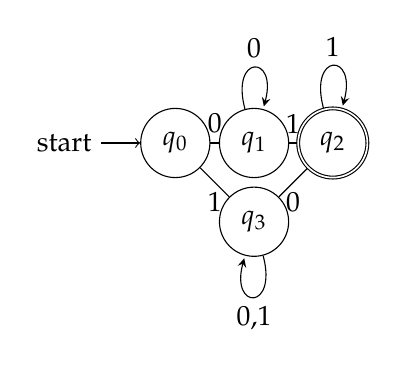
\begin{tikzpicture}
	\node[state, initial] (q0) {$q_0$};
	\node[state, right of=q0] (q1) {$q_1$};
	\node[state, accepting, right of=q1] (q2) {$q_2$};
	\node[state, below of=q1] (q3) {$q_3$};
	
	\draw [>=stealth] (q0) edge[above] node{0} (q1)
	      (q0) edge[below] node{1} (q3)
	      (q1) edge[loop above] node{0} (q1)
	      (q1) edge[above] node{1} (q2)
	      (q2) edge[below] node{0} (q3)
	      (q2) edge[loop above] node{1} (q2)
	      (q3) edge[loop below] node{0,1} (q3);
	\end{tikzpicture} 
	\end{center}

	The initial state of the machine is $q_0$. To check whether a word is ``accepted'' by a DFA, we simply need to follow the arrows from the initial state. This DFA works on strings of binary characters. For example, for ``001'', we would start in $q_0$, follow the arrow to $q_1$, then $q_1$ again, then to $q_2$. The inner circle for $q_2$ means that it is an \emph{accepting} state. If we end up in an accepting after processing all symbols in the input, the word is accepted by the DFA. In this case, ``001'' is accepted, but \emph{e.g.} ``0010'' would not be. In general, this DFA accepts all words comprised of one or more 0s followed by one or more 1s.

	\begin{subparts}
		\subpart[2] Define a type \haskellIn{State} which enumerates states of the DFA shown above and a type \haskellIn{Symbol} which enumerates symbols of the binary alphabet so that, for example, \haskellIn{Q0 :: State} and \haskellIn{ZERO :: Symbol}. \droppoints 
		
		\begin{solution}
			\emph{Application. 1 mark per definition.}
			\begin{verbatim}
			data State = Q0 | Q1 | Q2 | Q3 
			data Symbol = ZERO | ONE
			\end{verbatim}
		\end{solution}
		
		\subpart[4] Define a closed type family whose kind signature is given by
		\begin{center}
			\haskellIn{Delta :: State -> Symbol -> State}
		\end{center}
		and which implements transitions between states of the above DFA. For example, \haskellIn{Delta Q1 ONE} should reduce to \haskellIn{Q2}. \droppoints 
		
		\begin{solution}
			\emph{Application.}
			\begin{verbatim}
			type family Delta (q :: Q) (e :: E) :: Q where 
			    Delta Q0 ONE  = Q3 
			    Delta Q0 ZERO = Q1 
			    Delta Q1 ONE  = Q2 
			    Delta Q1 ZERO = Q1
			    Delta Q2 ONE  = Q2 
			    Delta Q2 ZERO = Q3 
			    Delta Q3 ONE  = Q3 
			    Delta Q3 ZERO = Q3
			\end{verbatim}
		\end{solution}
	
		\subpart[4] With the help of \haskellIn{Delta}, define a closed type family whose kind signature is given by
		\begin{center}
			\haskellIn{DeltaHat :: State -> [Symbol] -> State}
		\end{center}
		and which performs transitions for every symbol in a list of symbols, starting from a given initial state. For example, the type \linebreak \haskellIn{DeltaHat Q0 '[ZERO, ZERO, ONE]} should reduce to \haskellIn{Q2}. \droppoints 
		
		\begin{solution}
			\emph{Application.}
			\begin{verbatim}
			type family DeltaHat 
			  (q :: State) (e :: [Symbol]) :: State where 
			  DeltaHat q '[] = q 
			  DeltaHat q (e ': es) = DeltaHat (Delta q e) es
			\end{verbatim}
		\end{solution}
	
		\ifprintanswers \else \pagebreak \fi
	
		\subpart[8] Define a closed type family whose kind signature is given by 
		\begin{center}
			\haskellIn{Accepts :: State -> [State] -> [Symbol] -> Bool}
		\end{center}
		which determines whether a DFA accepts a given word. The first argument represents the initial state of the DFA, the second represents the list of final states, and the third argument represents the input word. For example, \haskellIn{Accepts Q0 '[Q2] '[ZERO, ZERO, ONE]} should reduce to \haskellIn{True}.
		\droppoints 
		
		\begin{solution}
			\emph{Application.}
			\begin{verbatim}
			type family Elem (x :: k) (xs :: [k]) :: Bool where 
			    Elem x '[]       = False 
			    Elem x (x ': xs) = True 
			    Elem x (y ': xs) = Elem x xs
			
			type family Accepts 
			    (q :: Q) (fs :: [Q]) (w :: [E]) :: Bool where 
			    Accepts q fs w = Elem (DeltaHat q w) fs
			\end{verbatim}
		\end{solution}
		
		\subpart[3] Define a proxy type for symbols and explain the need for proxy types in Haskell. \droppoints 
		
		\begin{solution}
			\emph{Application+Comprehension. 1 mark for definition, 2 marks for explanation.} Types in Haskell are erased during compilation once they have been checked and are therefore unavailable at run-time. As a result, functions only accept arguments whose types are of kind \haskellIn{*}. Proxy types are used to ``carry'' types of other kinds into the scope of a function's type.
			
			\begin{verbatim}
			data SProxy (s :: Symbol) = SProxy
			\end{verbatim}
		\end{solution}
		
		\subpart[4] Define a suitable type class and suitable type class instances to reify type-level symbols. \droppoints 
		
		\begin{solution}
			\emph{Application.} 
			\begin{verbatim}
			class ReifySymbol (q :: E) where 
			    reifySymbol :: SProxy q -> E
			
			instance ReifySymbol ZERO where 
			    reifySymbol _ = ZERO 
			
			instance ReifySymbol ONE where 
			    reifySymbol _ = ONE
			\end{verbatim}
		\end{solution}
		
	\end{subparts}
\end{parts}
 
	\end{questions}

	\pagebreak
	%\newpage

%\begin{center}
%	\vspace*{4cm}
%	\textbf{This page is intentionally left almost blank.}
%\end{center}

%\newpage

\begin{multicols}{2}\scriptsize 
	
	\textbf{\normalsize Appendix: Prelude}
	
	\begin{verbatim}
	class Eq a where
	  (==), (/=) :: a -> a -> Bool
	  x /= y = not (x == y)
	\end{verbatim}
	
	\begin{verbatim}
	class Eq a => Ord a where
	  (<), (<=), (>), (>=) :: a -> a -> Bool
	  min, max             :: a -> a -> Bool
	
	  min x y | x <= y    = x
	          | otherwise = y
	
	  max x y | x <= y    = y
	          | otherwise = x
	\end{verbatim}
	
	\begin{verbatim}
	class Enum a where
	  succ           :: a -> a 
	  pred           :: a -> a
	  toEnum         :: Int -> a
	  fromEnum       :: a -> Int 
	\end{verbatim}
	
	\begin{verbatim}
	class Bounded a where
	  minBound :: a 
	  maxBound :: a
	\end{verbatim}
	
	\begin{verbatim}
	class Num a where 
	  (+), (-), (*) :: a -> a -> a
	  negate        :: a -> a
	  abs           :: a -> a
	  signum        :: a -> a
	  fromInteger   :: Integer -> a
	\end{verbatim}
	
	\begin{verbatim}
	class Enum a => Integral a where 
	  quot      :: a -> a -> a
	  rem       :: a -> a -> a
	  div       :: a -> a -> a
	  mod       :: a -> a -> a
	  quotRem   :: a -> a -> (a, a)
	  divMod    :: a -> a -> (a, a)
	  toInteger :: a -> Integer
	\end{verbatim}
	
	\begin{verbatim}
	class Num a => Fractional a where
	  (/)          :: a -> a -> a
	  recip        :: a -> a
	  fromRational :: Rational -> a
	\end{verbatim}
	
	\begin{verbatim}
	data Int = ...
	  deriving ( Eq, Ord, Show, Read
	           , Num, Integral )
	\end{verbatim}
	
	\begin{verbatim}
	data Integer = ...
	  deriving ( Eq, Ord, Show, Read
	           , Num, Integral )
	\end{verbatim}
	
	\begin{verbatim}
	data Float = ...
	  deriving ( Eq, Ord, Show, Read
	           , Num, Fractional )
	\end{verbatim}
	
	\begin{verbatim}
	data Double = ...
	  deriving ( Eq, Ord, Show, Read
	           , Num, Fractional )
	\end{verbatim}
	
	\begin{verbatim}
	even :: Integral a => a -> Bool 
	even n = n `mod` 2 == 0
	\end{verbatim}
	
	\begin{verbatim}
	odd :: Integral a => a -> Bool 
	odd = not . even
	\end{verbatim}
	
	\begin{verbatim}
	class Show a where
	  show :: a -> String
	\end{verbatim}
	
	\begin{verbatim}
	class Read a where 
	  read :: String -> a
	\end{verbatim}
	
	\begin{verbatim}
	class Foldable t where
	  foldr   :: (a -> b -> b) -> b -> t a -> b
	  foldl   :: (b -> a -> b) -> b -> t a -> b
	  foldr1  :: (a -> a -> a) -> t a -> a
	  foldl1  :: (a -> a -> a) -> t a -> a
	  
	  null :: t a -> Bool 
	  null = foldr (\_ _ -> False) True
	  
	  length :: t a -> Int
	  length = foldr (\x r -> 1 + r) 0
	  
	  elem :: Eq a -> a -> t a -> Bool 
	  elem x = foldr (\y r -> x==y || r) False
	  
	  maximum :: Ord a => t a -> a 
	  maximum = foldl1 max
	  
	  minimum :: Ord a => t a -> a 
	  minimum = foldl1 min
	  
	  sum :: Num a => t a -> a 
	  sum = foldl (+) 0
	  
	  product :: Num a => t a -> a
	  product = foldl (*) 1
	\end{verbatim}
	
	\begin{verbatim}
	(.) :: (b -> c) -> (a -> b) -> a -> c
	(.) f g x = f (g x)
	\end{verbatim}
	
	\begin{verbatim}
	id :: a -> a
	id x = x
	\end{verbatim}
	
	\begin{verbatim}
	const :: a -> b -> a
	const x _ = x
	\end{verbatim}
	
	\begin{verbatim}
	($!) :: (a -> b) -> a -> b
	f $! x = ...
	\end{verbatim}
	
	\subsection*{Functors}
	
	\begin{verbatim}
	class Functor f where 
	  fmap :: (a -> b) -> f a -> f b
	\end{verbatim}
	\begin{displaymath}
	\begin{array}{lrcl}
	\textbf{Identity} & \mathit{fmap}~\mathit{id} & = &  \mathit{id} \\
	\textbf{Fusion} & \mathit{fmap}~(f \circ g) & = & \mathit{fmap}~f \circ \mathit{fmap}~g
	\end{array}
	\end{displaymath}
	
	\subsection*{Applicatives}
	
	\begin{verbatim}
	class Functor f => Applicative f where 
	  pure  :: a -> f a
	  (<*>) :: f (a -> b) -> f a -> f b
	\end{verbatim}
	\begin{displaymath}
	\begin{array}{lr}
	\textbf{Identity} & \mathit{pure}~\mathit{id} <\!\!*\!\!> v = v \\ 
	\textbf{Homomorphism} & \mathit{pure}~f <\!\!*\!\!> \mathit{pure}~x \\& = \mathit{pure}~(f~x) \\
	\textbf{Interchange} & u <\!\!*\!\!> \mathit{pure}~y \\
	& = \mathit{pure}~(\$~y) <\!\!*\!\!> u \\
	\textbf{Composition} & \mathit{pure}~(\circ) <\!\!*\!\!> u <\!\!*\!\!> v <\!\!*\!\!> w  \\
	& = u <\!\!*\!\!> (v <\!\!*\!\!> w)
	\end{array}
	\end{displaymath}
	
	\subsection*{Monads}
	
	\begin{verbatim}
	class Applicative m => Monad m where 
	  return :: a -> m a
	  return = pure
	
	  (>>=) :: m a -> (a -> m b) -> m b
	\end{verbatim}
	
	\begin{displaymath}
	\begin{array}{lrcl}
	\textbf{Left identity} & \mathit{return}~a \bind f & = & f~a \\
	\textbf{Right identity} & m \bind \mathit{return} & = & m \\
	\textbf{Associativity} & (m \bind f) \bind g & = & \\ \multicolumn{2}{r}{ m \bind (\textbackslash x \to f~x \bind g)}
	\end{array}
	\end{displaymath}
	
	\subsection*{Booleans}
	
	\begin{verbatim}
	data Bool = True | False
	  deriving ( Bounded, Enum, Eq, Ord
	           , Read, Show )
	\end{verbatim}
	
	\begin{verbatim}
	not :: Bool -> Bool
	not True  = False
	not False = True
	\end{verbatim}
	
	\begin{verbatim}
	(&&) :: Bool -> Bool -> Bool
	True && True = True 
	_    && _    = False
	\end{verbatim}
	
	\begin{verbatim}
	(||) :: Bool -> Bool -> Bool
	False || False = False 
	_     || _     = True
	\end{verbatim}
	
	\begin{verbatim}
	and :: Foldable t => t Bool -> Bool 
	and = foldr (&&) True
	\end{verbatim}
	
	\begin{verbatim}
	or :: Foldable t => t Bool -> Bool 
	or = foldr (||) False
	\end{verbatim}
	
	\begin{verbatim}
	all :: Foldable t => 
	       (a -> Bool) -> t a -> Bool
	all p = and . foldr (\x xs -> p x : xs) []
	\end{verbatim}
	
	\begin{verbatim}
	any :: Foldable t => 
	       (a -> Bool) -> t a -> Bool
	any p = or . foldr (\x xs -> p x : xs) []
	\end{verbatim}
	
	\begin{verbatim}
	otherwise :: Bool
	otherwise = True
	\end{verbatim}
	
	\subsection*{Characters} 
	
	\begin{verbatim}
	data Char = ...
	\end{verbatim}
	
	\begin{verbatim}
	type String = [Char]
	\end{verbatim}
	
	\begin{verbatim}
	isLower :: Char -> Bool 
	isLower c = c >= 'a' && c <= 'z'
	\end{verbatim}
	
	\begin{verbatim}
	isUpper :: Char -> Bool 
	isUpper c = c >= 'A' && c <= 'Z'
	\end{verbatim}
	
	\begin{verbatim}
	isAlpha :: Char -> Bool 
	isAlpha c = isLower c || isUpper c
	\end{verbatim}
	
	\begin{verbatim}
	isDigit :: Char -> Bool 
	isDigit c = c >= '0' && c <= '9'
	\end{verbatim}
	
	\begin{verbatim}
	isAlphaNum :: Char -> Bool 
	isAlphaNum c = isAlpha c || isDigit c
	\end{verbatim}
	
	\begin{verbatim}
	isSpace :: Char -> Bool 
	isSpace c = c `elem` " \t\n"
	\end{verbatim}
	
	\begin{verbatim}
	ord :: Char -> Int 
	ord c = ...
	\end{verbatim}
	
	\begin{verbatim}
	chr :: Int -> Char 
	chr n = ...
	\end{verbatim}
	
	\begin{verbatim}
	digitToInt :: Char -> Int 
	digitToInt c | isDigit c = ord c - ord '0'
	\end{verbatim}
	
	\begin{verbatim}
	intToDigit :: Int -> Char 
	intToDigit n 
	  | n >= 0 && n <= 9 = chr (ord '0' + n)
	\end{verbatim}
	
	\begin{verbatim}
	toLower :: Char -> Char 
	toLower c 
	  | isUpper c =
	      chr (ord c - ord 'A' + ord 'a')
	  | otherwise = c
	\end{verbatim}
	
	\begin{verbatim}
	toUpper :: Char -> Char 
	toUpper c 
	  | isLower c =
	      chr (ord c - ord 'a' + ord 'A')
	  | otherwise = c
	\end{verbatim}
	
	\subsection*{Lists}
	
	\begin{verbatim}
	data [a] = [] | (:) a [a]
	  deriving (Eq, Ord, Show, Read)
	\end{verbatim}
	
	\begin{verbatim}
	instance Functor [] where 
	  fmap = map
	\end{verbatim}
	
	\begin{verbatim}
	instance Applicative [] where
	  pure x = [x]
	  
	  fs <*> xs = [f x | f <- fs, x <- xs]
	\end{verbatim}
	
	\begin{verbatim}
	instance Monad [] where 
	  xs >>= f = [y | x <- xs, y <- f x]
	\end{verbatim}
	
	\begin{verbatim}
	instance Foldable [] where 
	  foldr _ v []     = v 
	  foldr f v (x:xs) = f x (foldr f v xs)
	  
	  foldr1 _ [x]    = x 
	  foldr1 f (x:xs) = f x (foldr1 f xs)
	  
	  foldl _ v []     = v 
	  foldl f v (x:xs) = foldl f (f v x) xs
	  
	  foldl1 f (x:xs) = foldl f x xs
	\end{verbatim}
	
	\begin{verbatim}
	head :: [a] -> a 
	head (x:xs) = x
	
	tail :: [a] -> [a]
	tail (x:xs) = xs
	\end{verbatim}
	
	\begin{verbatim}
	last :: [a] -> a
	last [x]    = x
	last (x:xs) = last xs
	\end{verbatim}
	
	\begin{verbatim}
	init :: [a] -> [a]
	init [_]    = []
	init (x:xs) = x : init xs
	\end{verbatim}
	
	\begin{verbatim}
	map :: (a -> b) -> [a] -> [b]
	map f []     = []
	map f (x:xs) = f x : map f xs
	\end{verbatim}
	
	\begin{verbatim}
	filter :: (a -> Bool) -> [a] -> [a]
	filter p [] = []
	filter p (x:xs)
	  | p x       = x : filter p xs
	  | otherwise = filter p xs
	\end{verbatim}
	
	\begin{verbatim}
	lookup :: Eq k => k -> [(k,v)] -> Maybe v
	lookup x [] = Nothing
	lookup x ((y,v):ys)
	  | x == y    = Just v
	  | otherwise = lookup x ys
	\end{verbatim}
	
	\begin{verbatim}
	(!!) :: [a] -> Int -> a
	(x:xs) !! 0 = x
	(x:xs) !! n = xs !! (n-1)
	\end{verbatim}
	
	\begin{verbatim}
	take :: Int -> [a] -> [a]
	take 0 _      = []
	take n []     = []
	take n (x:xs) = x : take (n-1) xs
	\end{verbatim}
	
	\begin{verbatim}
	drop :: Int -> [a] -> [a]
	drop 0 xs     = xs 
	drop n []     = []
	drop n (x:xs) = drop (n-1) xs
	\end{verbatim}
	
	\begin{verbatim}
	takeWhile :: (a -> Bool) -> [a] -> [a]
	takeWhile _ [] = []
	takeWhile p (x:xs) 
	  | p x       = x : takeWhile p xs
	  | otherwise = []
	\end{verbatim}
	
	\begin{verbatim}
	dropWhile :: (a -> Bool) -> [a] -> [a]
	dropWhile _ [] = []
	dropWhile p (x:xs) 
	  | p x       = dropWhile p xs
	  | otherwise = x : xs
	\end{verbatim}
	
	\begin{verbatim}
	splitAt :: Int -> [a] -> ([a], [a])
	splitAt n xs = (take n xs, drop n xs)
	\end{verbatim}
	
	\begin{verbatim}
	span :: (a -> Bool) -> [a] -> ([a], [a])
	span p xs = 
	  (takeWhile p xs, dropWhile p xs)
	\end{verbatim}
	
	\begin{verbatim}
	repeat :: a -> [a]
	repeat x = xs where xs = x : xs
	\end{verbatim}
	
	\begin{verbatim}
	replicate :: Int -> a -> [a]
	replicate n = take n . repeat
	\end{verbatim}
	
	\begin{verbatim}
	iterate :: (a -> a) -> a -> [a]
	iterate f x = x : iterate f (f x)
	\end{verbatim}
	
	\begin{verbatim}
	zip :: [a] -> [b] -> [(a,b)]
	zip []     _      = []
	zip _      []     = []
	zip (x:xs) (y:ys) = (x,y) : zip xs ys
	\end{verbatim}
	
	\begin{verbatim}
	(++) :: [a] -> [a] -> [a]
	[]     ++ ys = ys
	(x:xs) ++ ys = x : (xs ++ ys)
	\end{verbatim}
	
	\begin{verbatim}
	concat :: [[a]] -> [a]
	concat = foldr (++) []
	\end{verbatim}
	
	\begin{verbatim}
	reverse :: [a] -> [a]
	reverse = foldl (\xs x -> x : xs) []
	\end{verbatim}
	
	\begin{verbatim}
	subsequences :: [a] -> [[a]]
	subsequences []     = [[]]
	subsequences (x:xs) = ys ++ map (x:) ys
	  where ys = subsequences xs
	\end{verbatim}
	
	\begin{verbatim}
	nub :: Eq a => [a] -> [a]
	nub []     = []
	nub (x:xs) = x : nub (filter (/= x) xs)
	\end{verbatim}
	
	\begin{verbatim}
	delete :: Eq a => a -> [a] -> [a]
	delete _ []     = []
	delete x (y:ys) 
	  | x == y    = ys
	  | otherwise = y : delete x ys
	\end{verbatim}
	
	\subsection*{Maybe}
	
	\begin{verbatim}
	data Maybe a = Nothing | Just a
	  deriving (Eq, Ord, Read, Show)
	\end{verbatim}
	
	\begin{verbatim}
	instance Functor Maybe where
	  fmap f Nothing  = Nothing
	  fmap f (Just x) = Just (f x)
	\end{verbatim}
	
	\begin{verbatim}
	instance Applicative Maybe where
	  pure x = Just x
	  
	  Nothing  <*> _ = Nothing
	  (Just f) <*> y = fmap f y
	\end{verbatim}
	
	\begin{verbatim}
	instance Monad Maybe where
	  Nothing  >>= f = Nothing
	  (Just x) >>= f = f x
	\end{verbatim}
	
	\subsection*{Either}
	
	\begin{verbatim}
	data Either a b = Left a | Right b
	\end{verbatim}
	
	\subsection*{Tuples}
	
	All tuples are instances of \texttt{Eq}, \texttt{Ord}, \texttt{Show}, \texttt{Read}.
	
	\begin{verbatim}
	fst :: (a, b) -> a
	fst (x,y) = x
	\end{verbatim}
	
	\begin{verbatim}
	snd :: (a, b) -> b
	snd (x,y) = y
	\end{verbatim}
	
	\begin{verbatim}
	curry :: ((a, b) -> c) -> a -> b -> c 
	curry f x y = f (x, y)
	\end{verbatim}
	
	\begin{verbatim}
	uncurry :: (a -> b -> c) -> (a, b) -> c
	uncurry f (x,y) = f x y
	\end{verbatim}
	
	\subsection*{IO}
	
	\begin{verbatim}
	data IO a = ...
	
	instance Functor IO where ...
	instance Applicative IO where ...
	instance Monad IO where ...
	\end{verbatim}
	
	\begin{verbatim}
	getChar :: IO Char
	getChar = ...
	
	getLine :: IO String
	getLine = ...
	
	putChar :: Char -> IO ()
	putChar c = ...
	
	putStr :: String -> IO ()
	putStr []     = return ()
	putStr (x:xs) = putChar x >> putStr xs
	
	putStrLn :: String -> IO ()
	putStrLn xs = putStr xs >> putChar '\n'
	
	print :: Show a => a -> IO ()
	print = putStrLn . show
	\end{verbatim}
	
	\subsection*{Type-level programming}
	
	The kind of types is denoted as \texttt{*}. 
	
	\begin{verbatim}
	data Nat = Zero | Succ Nat
	\end{verbatim}
\end{multicols}

\end{document}